\documentclass{mldsmsc}

\title{Deep Reinforcement Learning for Ad Personalization}
\author{Martin Bat\v{e}k}
\CID{00951537}
\supervisor{Mikko Pakkanen}
\date{2 September 2024}
%For today's date, use:
%\date{\today}
\logoimg{}


% THIS IS WHERE NEW COMMANDS CAN BE DEFINED
% commands below only used in the proof; otherwise can be deleted
\newcommand{\consta}{a}
\newcommand{\X}{X}
\newcommand{\EE}[1]{ \mathrm{E} [ #1 ] }
\newcommand{\inparenth}[1]{\left( #1 \right)}

\begin{document}

% Generates the Title Page
\maketitle


% Generates plagiarism declaration
\declarationname{Martin Bat\v{e}k}
\declarationdate{17 July 2024}
\declaration 


\begin{abstract}
    ABSTRACT GOES HERE
\end{abstract}

\begin{acknowledgements}
    ANY ACKNOWLEDGEMENTS GO HERE
\end{acknowledgements}

% add glossary?

% table of contents
\tableofcontents

% VERY IMPORTANT
% This command switches from Roman to Arabic numbering for main part of thesis
\mainmatter


\chapter{Introduction}

The global digital advertising market is worth approximately \$602 billion today. Due to the increasing rate of of online participation since the 
COVID-19 pandemic, this number has been rapidly increasing and is expected to reach \$871 billion by the end of 2027 \citep{RefWorks:emarketer2023digital}.
Many of the of the major Ad platforms such as Google, Facebook and Amazon operate on a cost-per-user-engagement pricing model, which usually means that 
advertisers get charged for every time a user clicks on an advertisment. This means that there is
a significant commercial incentive to design Ad-serving platforms that ensure that the content 
shown to each user is as relevent as possible, so as to maximize user engagement and platform revenues
as much as possible.

\begin{figure}[h]
\centering
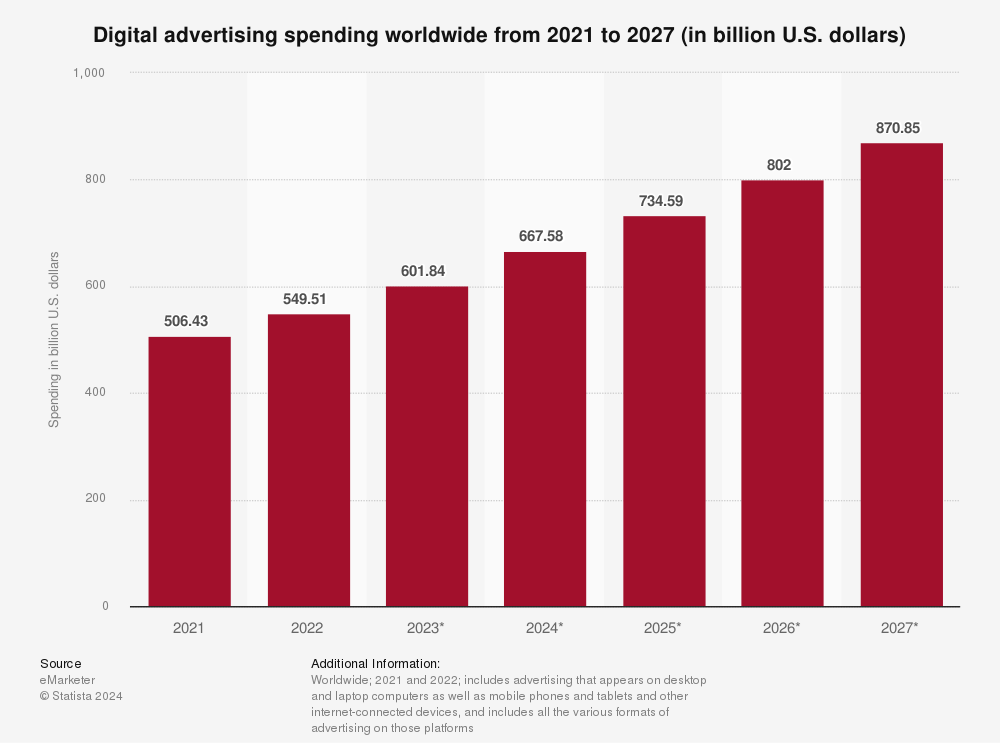
\includegraphics[width=0.8\textwidth]{../figures/eMarketer - Ad Spending.png}
\caption{Global Digital Ad Spending 2021-2027. Image taken from \cite{RefWorks:emarketer2023digital}}
\label{fig:ad-spending}
\end{figure}

Attaining accurate Click-Through Rate (CTR) 
prediction is a necessary first step for Ad persionalization, which is why study of CTR prediction methods have been an extremely active part of 
Machine Learning research over the past through years. Initially, shallow prediction methods such as Logistic Regression, Factorization Machines \citep{RefWorks:rendle2010factorization} and Field-Aware Factorization 
Machines \citep{RefWorks:juan2016field-aware} have been used for CTR prediction. However, these methods have often been shown to be unable to capture the 
higher order feature interactions in the sparse multi-value categorical Ad Marketplace datasets \citep{RefWorks:zhang2021deep}. Since then, Deep Learning methods have been 
shown to show superior predictive ability on these datasets. A number of Deep Learning models have been proposed, each using a
different techniques for feature interaction modelling, ranging from Deep Learning extensions of Factorization Machines
such as DeepFM \citep{RefWorks:guo2017deepfm:}, to novel methods such as AutoInt \citep{RefWorks:song2019autoint}. By employing a
multi-towered neural network architecture, these models are able to capture both low-order and high-order feature interactions in the data,
and therefore tend to achieve supperior predictive performance to their shallow counterparts.

However, irrespective of how well these models perform in a static environments, the reality is that user preferences
and advertisment characteristics are constantly changing. Like most online reccomender systems,
Ad personalization models must be able to adapt to these changes in order to continue to provide accurate predictions 
over the longer period \citep{RefWorks:zheng2018drn:}. This problem necessitates the use
of Reinforcement Learning for Ad personalization.

Reinforcement Learning is a subdomain of Machine Learning in which the goal is for an agent to
learn an optimal policy that maximizes the expected reward in an environment where the
state-action-reward progression can be modelled as a Markov Decision Process
\citep{puterman2014markov}. Early Reinforcement Learning methods involved 
deriving a the transition probabilities for the state-action pairs on the basis of interactions
with the environment and then using Dynamic Programming methods such as the Upper Confidence
Bound RL (UCB-RL) algorithm \citep{RefWorks:auer2008near-optimal} and the
the Thompson Sampling algorithm for Reinforcement Learning \citep{RefWorks:pike-burke2024optimism/thompson}.
However, in cases where the state-action space is too sparce to be
reasonably enumerated, it is often more practical to user a function approximator 
to directly estimate the expacted cumalative reward for each action in each state. This method of Reinfocement
Learning is commonly referred to as Q-learning \citep{RefWorks:watkins1989learning},
and has the advantage of being \emph{model-free}, meaning that
it does not require the agent to have a model of the environment
thereby making it more scalable to large and sparce datasets. In \citep{RefWorks:hornik1989multilayer},
\citep{RefWorks:cybenko1989approximation} and \citep{RefWorks:hornik1990universal} Deep
Neural Networks with activation functions are shown to be universal function approximators
which naturally lead to the incorporation of DNN's in Q-Learning. This has lead to the
development of the Deep Q-Learning Agent, which has been shown to be able to learn optimal
policies in a number of different domains, such as the Atari 2600 game environment \cite{RefWorks:mnih2015human-level}.
Beyond this, Deep Reinforcement Learning has shown promising results in a number
of different aplications, including robot control and computer vision \citep{RefWorks:wang2024deep}.
In the context of Ad personalization, DRL has also be applied to online reccomender systems
such as News article reccomendation \citep{RefWorks:zheng2018drn:} and video
reccomendation on Youtube \citep{RefWorks:chen2019top-k}. In both papers,
the authors show that the DRL agent is able to learn an optimal content reccomendation
policy on the basis of user engagement data. This reveals that there is potential
for applying these methods to the problem of Ad personlization, thereby creating a 
truely adaptive marketing platform.

\subsubsection{Research Question and Contributions}

In this report, I aim to construct a Ad serving system that is truely adaptive and 
personalized to the changing user preferences and advertisment charateristics. In order
to achieve this goal, I will first need to find a suitable Deep Learning Model arcitecture
for CTR prediction, and then incorporating this model as the Q-function approximator in
a Deep Q-Learning algorithm. The key contributions that I make in this report are as follows:

\begin{itemize}
\item I evaluate the performance of five popular Deep Learning models for CTR prediction on three well-known benchmark datasets, Criteo \citep{RefWorks:tien2014display}, KDD12 \citep{RefWorks:aden2012kdd} and Avazu \citep{RefWorks:wang2014click-through}.
\item I construct a novel Deep Reinforcement Learning Frame for Ad personalization, and as a proof-of-concept and evaluate its performance using the KDD12 dataset.
\end {itemize}

\subsubsection{Structure of the Report}

In chapter~\ref{chap:background}, I begin by providing a background introducing the problem
of Click-Through Rate prediction in the context of Ad personalization, and explore the unique challenges posed 
by the typically sparse multi-value categorical datasets that are common in the Ad marketplace. I then 
proceed to review the literature on Deep Learning models for CTR prediction, highlighting
the different techniques that each framework uses to capture the key feature interactions in the data. 
I also review the literature on Deep Reinforcement
Learning, specifically the DRN algorithm introduced by \cite{RefWorks:zheng2018drn:}, which can be analogously
applied to the Ad personalization context. In chapter \ref{chap:deep-ctr-model-evaluation}, I evaluate the performance of different
Deep Learning models for CTR prediction on three well-known benchmark datasets, Criteo \citep{RefWorks:tien2014display}, KDD12 \citep{RefWorks:aden2012kdd} 
and Avazu \citep{RefWorks:wang2014click-through}. In chapter~\ref{chap:deep-rl-for-ad-personalization}, I construct a Deep Reinforcement Learning model for Ad personalization and evaluate its performance
on the same benchmark datasets. Finally, in chapter~\ref{chap:discussion}, I discuss the results of the experiments and provide some concluding remarks.

\chapter{Background}
\label{chap:background}

\section{Deep CTR Prediction}

\subsection{Problem Formulation and Ad Marketplace Data}
\label{sec:problem-formulation-data}

In their respective surveys on the use of Deep Learning methods for CTR prediction, \cite{RefWorks:gu2021ad} 
and \cite{RefWorks:zhang2021deep} outline the problem of CTR prediction as one that essentially boils down to
a binary (click/no-click) classification problem utilizing user/ad-view event level online session records. 
The goal of CTR prediction is to train a function $f$ that takes in a set of ad marketplace 
features $\mathbf{x} \in \mathbb{R}^n$, and maps these to a probability that the user 
will click on the ad in that given context. In other words, $f_{\Theta}: \mathbb{R}^n \rightarrow \mathbb{R}$ such that:

\begin{equation}
\label{eqn:ctr-classifier}
\mathbb{P}(\text{click}| \mathbf{x})
= \mathbb{P}(y = 1 | \mathbf{x})
= \sigma(f_{\Theta}(\mathbf{x}))
\end{equation}

where $y$ is the binary click label, $\Theta$ represents the parameter vector for $f$ and
$\sigma(x)=(1 + e^{-x})^{-1}$ is the sigmoid function. To ease the notation for the rest of the report,
we will use the shorthand $p(y) = \mathbb{P}(y=1 | \mathbf{x})$ formulations in the following
sections. 

An instance of the ad marketplace features $\mathbf{x}$ is typically
recorded at a user/ad impression event level and typically consists of

\begin{itemize}
\item \textbf{User Features:} Features that describe the user, such as User ID, demographic information,
metrics related to the user's past interactions with the platform, etc.
\item \textbf{Ad Features:} Features that describe the ad, such as Ad ID, Advertiser ID and Ad Category.
\item \textbf{Contextual Features:} Features that describe the context in which the ad is being shown, such as
the time of day, the position of the ad on the page and the site on which the ad is being shown.
\end{itemize}

\begin{figure}[h]
\centering
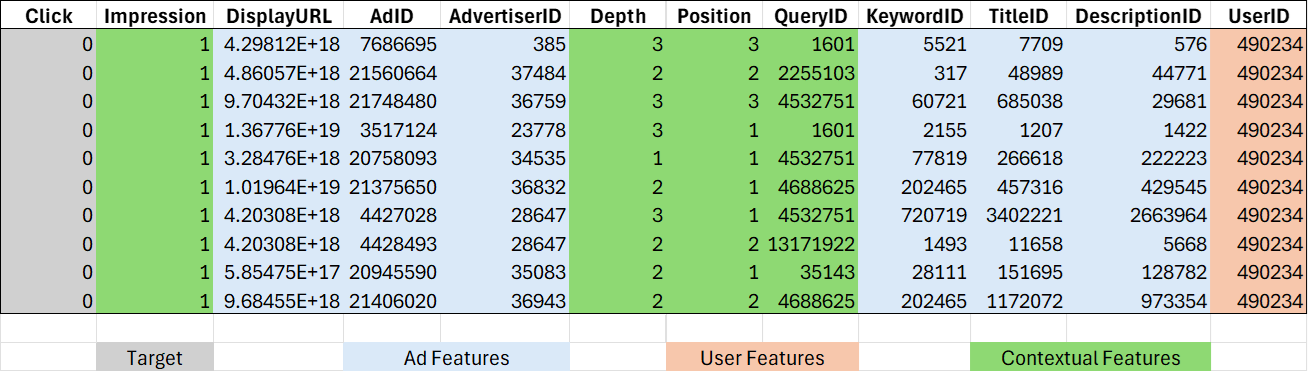
\includegraphics[width=0.8\textwidth]{../figures/kdd12_snapshot.png}
\caption{Snapshot of the KDD12 dataset \cite{RefWorks:aden2012kdd}}
\label{fig:kdd12-snapshot}
\end{figure}

Figure~\ref{fig:kdd12-snapshot} shows a snapshot of the KDD12 dataset, which is a typical example of 
the type of data that is used for CTR prediction.

A defining characteristic for this type of data is that many of the features are multi-value categories with 
a high degree of of cardinality \citep{RefWorks:he2017neural}. In order to user categorical data
in a classifier model, it is common practice to embed the these categorical features
as multidimensional vectors. While the dimensionality of these embeddings can vary amongt the different
sparse categorical features, for the sake of simplicity of notation, below we assume that all sparse categorical feature
embeddings have the same dimensionality, $D$. Let $\mathbf{x_i}^{OH}$ be the one-hot encoded vector
representation of the categiorical feature $x_i$. Then the \emph{embedded} feature vector
$\mathbf{e}_i$ for categorical feature $x_i$ is given by:

\begin{equation}
\label{eqn:cat-embedding}
\begin{split}
\mathbf{e}_i &= \mathbf{B}_i \mathbf{x}_i^{OH}\\
&= \left[\mathbf{b}_{1}^{i}, \ldots, \mathbf{b}_{m_i}^{i} \right] \mathbf{x}_i^{OH} \\
&= \begin{bmatrix}
b_{1,1}^i & \cdots & b_{1 ,C_i}^i\\
\vdots & \ddots & \\
b_{D, 1}^i & \cdots & b_{D, C_i}^i
\end{bmatrix}
\begin{bmatrix}
    0 \\
    \vdots \\
    1 \\
    0\\
    \vdots
\end{bmatrix}
\end{split}
\end{equation}

where $\mathbf{B}_i$ is the embedding matrix for feature $x_i$, whose dimensions are determined
by the chosen embedding dimension $D$ and the cardinality of the feature, $C_i$. Assuming
that value of $x_i$ is equal to the $k$-th value in the one-hot encoding mapping, and that therefore
the $k$-th value in $\mathbf{x}_i^{OH}$ is equal to one, Equation~\ref{eqn:cat-embedding} then simplifies
to

\begin{equation}
    \mathbf{e}_i = \left[e_{i 1}, \ldots, e_{i, D} \right]^{\intercal}
    = \left[b_{1 k}^{i}, b_{2 k}^{i}, \ldots , b_{D k}^{i}\right]^{\intercal} = \mathbf{b}_{k}^{i}
\end{equation}

which is the $k$-th column of the embedding matrix $\mathbf{B}_i$, otherwise referred to as the $k$-th
embedding vector \citep{RefWorks:hancock2020survey}. The processed data $\tilde{\mathbf{x}}$ that then gets fed into the model is 
then composed of a concatenation of all sparse feature embeddigs $\mathbf{e}_i$ and standardized
dense numerical feature values
$z_i = (x_i - \bar{x_i})/\sqrt{Var(x_i)}$:

\begin{equation}
    \begin{split}
    \tilde{\mathbf{x}} &= \left[ \mathbf{e}_1^{\intercal}, \dots , \mathbf{e}_s^{\intercal}, z_{s+1}, \dots , z_{s+d} \right]\\
    &= \left[e_{1, 1}, \ldots, e_{1 ,D}, e_{2, 1}, \ldots , e_{s, D}, z_{s+1}, \ldots, z_{s+d}\right]\\
    &= \left[ \tilde{x}_1, \ldots, \tilde{x}_{\tilde{n}}\right]
    \end{split}
\end{equation}

where $s$ and $d$ are the number of \emph{sparse} categorical features and \emph{dense}
numerical features respectively in $\mathbf{x}$, and $\tilde{n} = D\cdot s + d$
is the resulting dimensionality of $\tilde{\mathbf{x}}$. Again, to ease the notation in the
remainder of the report, we will assume that the prepocessing steps described above
are applied to the data, and all formulaic expressions of the models in the following
section with be expressed in terms of $\tilde{\mathbf{x}} = \{\tilde{x}_j\}_{j=1}^{\tilde{n}}$.

The problem posed by high cardinality is that when $m_i$ is large, the high
sparsity of the one-hot encoded vector $x_i^{OH}$ can make in extremely difficult
for a model to learn the key \emph{implicit} features and patterns present in the
data \citep{RefWorks:gu2021ad}. This is indeed the key challenge in building an
accurate CTR prediction model, and is a key motivating factor as to why Deep Neural
networks have out performed the classical shallow counterparts. This transition will be examined
in more detail in the following section.

\subsection{Shallow CTR Models}

\subsubsection{Logistic Regression}

The earliest examples of CTR classification models incorporated classical ``shallow'' 
(single layer) statistical regression methods. The most basic example of this was 
the \textbf{Logistic Regression} model, as implemented by \cite{RefWorks:richardson2007predicting} on
advistisment data from the Microsoft Search engine. The LR model
is composed by modelling the \emph{log-odds} (also referred to as the \emph{logit}) 
of a positive binary label as a linear combination
of all of the respective feature values:

\begin{equation}
\label{eqn:lr-model}
f_{\Theta}^{LR}(\tilde{\mathbf{x}}) = \theta_0 + \sum_{j=1}^{\tilde{n}}\theta_j \tilde{x}_j
\end{equation}

where $f_{\Theta}^{LR}: \mathbb{R}^n \rightarrow \mathbb{R}$ represents the Logistic regression
model parametized by $\Theta = (\theta_0, \ldots, \theta_{\tilde{n}})$. The benefits of the LR
model are that due to its simplicity and low number of parameters, it is relatively easy to
train in computational terms and also relatively easy to deploy \citep{RefWorks:zhang2021deep}.
Howevever, the formulation in equation~\ref{eqn:lr-model} reveals that the LR model does not explicitly 
account for \emph{feature interactions}.
As outlined in section~\ref{sec:problem-formulation-data}, the categorical features tend to have a
high cardinality, resulting in highly sparse feature embeddings. Many of the of the important patterns
for CTR prediction are therefore likely to be expressed in terms of \emph{combinations of features}
rather then the individual feature values themselves. For example, a user's tendancy to
click on a given advertisment is likely to by influenced by the \emph{combination} of the category
of good or service the given advertisment is trying to sell (e.g. premium fashion retail, travel, electronics et. cetera)
and the demographic/socio-economic category that the given user falls into (e.g. university student, young professional, retiree).
These features combinations (and the corresponding combination of respective field values 
in the preprocessed feature vector $\tilde{\mathbf{x}}$) are commonly referred to in
the literature as \emph{cross-features} \citep{RefWorks:zhang2023memonet:} or more commonly
\emph{feature interactions} \citep{RefWorks:cheng2016wide,RefWorks:xiao2017attentional,RefWorks:song2019autoint}.

Whilst it is possible to incorporate feature interactions in an LR model through feature
engineering, this quickly becomes infeasible for large sparse datasets. A number of techniques
have been developed to automate the necessary feature engineering steps for this, either by
implicitly assigning a weight to all second order feature interactions \citep{RefWorks:chang2010training}
or by utilizing Gradient Boosted Decision Trees to pick out the key interactions \citep{RefWorks:cheng2014gradient}.
Unfortunately, the prior still tends to exhibit poor performance with sparse data, 
whereas the fact that the Gradient Boosting algorithm for the latter is difficult to paralellize
makes this solution difficult to scale in many applications in practice \citep{RefWorks:zhang2021deep}.

\subsubsection{Factorization Machines}

\textbf{Factorization Machines} first proposed by \cite{RefWorks:rendle2010factorization} can 
be thought of as an extension of the Logistic Regression framework in equation~\ref{eqn:lr-model}
with additional terms that explicitly account for the interactions between different features.
Its relative simplicity and computational scalability has made it a widely popular framework
for CTR modelling \citep{RefWorks:gu2021ad}. 
A 2-way (maximum feature interaction degree of 2) Factorization Machine model is formulated as:

\begin{equation}
\label{eqn:fm-2way}
f_{\Theta}^{FM^2}(\tilde{\mathbf{x}}) = \theta_0 + \sum_{j=1}^{\tilde{n}} \theta_{j} \tilde{x}_j
+ \sum_{j=1}^{\tilde{n}} \sum_{k=j+1}^{\tilde{n}} \langle \mathbf{v}_j , \mathbf{v}_k \rangle \tilde{x}_j \tilde{x}_k
\end{equation}

where $\langle \cdot , \cdot \rangle$ represents the inner product between two vectors, the final
interaction term above is parametized by $\mathbf{V} \in \mathbb{R}^{\tilde{n} \times F}$. Each
row $\mathbf{v}_j$ of $\mathbf{V}$ represents the $j$-th feature in $\tilde{\mathbf{x}}$ in terms
of $F$ latent factors. The factorization matrix $\mathbf{V}$ is typically fitted by optimizing
the binary cross-entropy loss function by means of Stochastic Gradient Descent. It is 
intutive to see that $\mathbf{V}$ will be fitted such that if the interaction
between feature $j$ and $k$ have a positive impact on $p(y)$, then $j$-th and 
$k$-th rows of $\mathbf{V}$ will have positive inner products (and vice versa) \citep{RefWorks:zhang2021deep}.

\cite{RefWorks:rendle2010factorization} shows that although direct evaluation
of equation~\ref{eqn:fm-2way} would appear to have a complexity of $O(F \tilde{n}^2)$, the 2-way
FM model in fact scales linearly in $\tilde{n}$ and $F$:

\begin{lemma}
\label{lemma:fm-linearity}
The model equation of a 2-way factorization machine (eq.~\ref{eqn:fm-2way}) can
be computed in linear time $O(L\tilde{n})$.
\end{lemma}

\begin{proof}
\label{prf:fm-linearity}

Due to the factorization of the pairwise interactions, there is no model
parameter that directly depends on two features $(j,k)$. This means that
pairwise interactions can be reformulated as such

\begin{align*}
    &\sum_{j=1}^{\tilde{n}} \sum_{k=j+1}^{\tilde{n}} \langle \mathbf{v}_j , \mathbf{v}_k \rangle \tilde{x}_j \tilde{x}_k \\
    &= \sum_{j=1}^{\tilde{n}} \sum_{k=j+1}^{\tilde{n}} 
    \sum_{f=1}^{F}v_{j,f} v_{k,f}\tilde{x}_j \tilde{x}_k \\
    &= \frac{1}{2} \left( \sum_{j=1}^{\tilde{n}} \sum_{k=1}^{\tilde{n}}
    \sum_{f=1}^{F} v_{j,f} v_{k,f} \tilde{x}_j \tilde{x}_k -
    \sum_{j=1}^{\tilde{n}} \sum_{f=1}^{F}v_{j,f} v_{j,f} \tilde{x}_j \tilde{x}_j \right)\\
    &=\frac{1}{2}\sum_{f=1}^{F} \left( \sum_{j=1}^{\tilde{n}}v_{j,f} \tilde{x}_j
    \sum_{k=1}^{\tilde{n}} v_{k,f} \tilde{x}_k - \sum_{j=1}^{\tilde{n}}
    v_{j,f}^2 \tilde{x}_j^2 \right)\\
    &= \frac{1}{2}\sum_{f=1}^{F} \left( \left(\sum_{j=1}^{\tilde{n}}v_{j,f} \tilde{x}_j\right)^2
    - \sum_{j=1}^{\tilde{n}} v_{j,f}^2 \tilde{x}_j^2 \right)
\end{align*}

The complexity of the final line above is $O(L\tilde{n})$, and hence the FM formulation
as per equation~\ref{eqn:fm-2way} scales linearly in $L$ and $\tilde{n}$.
\end{proof}

This quality greatly simplifies the computational complexity of scaling the FM model to larger
datasets with a more sparse categorical features. Morever, the Factorization Machine framework
can be generalized to degree $R$ (i.e. up to any limit of feature interation order) as follows:

\begin{multline}
\label{eqn:fm-rway}
f_{\Theta}^{FM^R} = \theta_0 + \sum_{j=1}^{\tilde{n}} \theta_{j} \tilde{x}_{j}
+ \sum_{r=1}^{R} \sum_{j_1=1}^{\tilde{n}} \cdots \sum_{j_r = j_{r-1} + 1}^{\tilde{n}}
\left( \prod_{k=1}^{r} \tilde{x}_{j_k} \right)
\left( \sum_{f = 1}^{F_r} \prod_{k=1}^{r} v_{j_k, f}^{(r)}\right)
\end{multline}

The FM framework therefore provides an intuitive and computationally scalable method to
account for key feature interactions without the need of extensive feature engineering. Extensions
and improvements to FM have been proposed, most notably in the form of
the Field-Aware Factorization Machine (FFM) framework by \cite{RefWorks:juan2016field-aware},
which only acounts for intereactions between features of different fields 
(in otherwords, it ignores the interaction between $\tilde{x}_j$ and $\tilde{x}_k$ if
both are componets of embedding vector $mathbf{e}_i$ for some categorical feature $x_i$)
as well as Gradient Boosted Factorization Machines \citep{RefWorks:cheng2014gradient}, 
which again aims to augment the FM framework by means of the Gradient Boosting algorithm.

\subsection{Introducing MLP's in CTR prediction}

Despite the advantages of the FM framework, a setback of the formulation in equation~\ref{eqn:fm-rway}
is that the framework grows highly compex and overparametized for higher values of $R$.
As a consequence, only the 2-way FM framework as per equation~\ref{eqn:fm-2way} tends to be
implemented in practice, meaning that in FM alone is feasably insufficient for capturing
feature interactions of order $>>2$ \citep{RefWorks:guo2017deepfm:}. Deep Neural Networks
present a powerful alternative for addressing this shortcoming. Neural networks benefit from
being universal function approximators \citep{RefWorks:cybenko1989approximation} and from the
fact that neural network batch training is paralelizable by means of GPU accelerated computation.
This has lead to the successfull application of Deep Learning algorithms across multiple fields
such as Natural Language Processing and Image classification 
\citep{RefWorks:he2016deep,RefWorks:krizhevsky2017imagenet,RefWorks:lecun1998gradient-based}. 
These factors and successes showed that DNN's have the potential to extract informative
feature representations from highly sparse and abstract data, and as a consequence,
the application of DNN's in CTR prediction started recieving attention in the mid-2010's.

The \textbf{Multilayer Perceptron} (MLP) \label{ref:mlp} is the most elementary type of Deep Neural Network
\citep{RefWorks:webster2024week}. In general, a MLP with $L$ hidden layers is formulated as such:

\begin{align}
\label{eqn:mlp}
\mathbf{h}^{(0)} &:= \tilde{\mathbf{x}} \\
\mathbf{h}^{(l)} &= \phi_{l} \left( \mathbf{W}^{(l-1)} + \mathbf{b}^{(l-1)} \right), l = 1, \ldots, L \\
\hat{y} &= \phi_{out} \left( \mathbf{w}^{(L)} \mathbf{h}^{(L)} + b^{(L)} \right)
\end{align}

where $\mathbf{W}^{(k)} \in \mathbb{R}^{n_{l+1} \times n_l } $, $\mathbf{b}^{(k)} \in \mathbf{R}^{n_{l+1}}$,
$\mathbf{h}^{(l)} \in \mathbb{n_l}$, $n_0 = \tilde{n}$, $n_l$ is the number of hidden
units in layer $l$ and $\phi_{l}$ is the activation function for layer $l$, 
When rearranged in the form of equation~\ref{eqn:ctr-classifier}, the above becomes:

\begin{equation}
\label{eqn:mlp-2}
f_{\Theta}^{MLP}(\tilde{\mathbf{x}}) = \psi_{out} \left( \psi_{L} \left( \cdots \psi_{1} \left( 
    \tilde{\mathbf{x}} \right) \cdots \right) \right)
\end{equation}

where each function $\psi_{l}$ represents the affine transformation and element-wise activation
operation for layer $l$. MLPs can be thought of as an acyclic graph, as displayed in
Figure~\ref{fig:mlp}. The data $\tilde{\mathbf{x}}$ first gets fed through the
\emph{input layer}, then gets processed by multiple \emph{hidden layers} that include
a series of affine transfromations followed by activation functions, before the final
result is produced by the \emph{output layer}.

\begin{figure}[h]
    \centering
    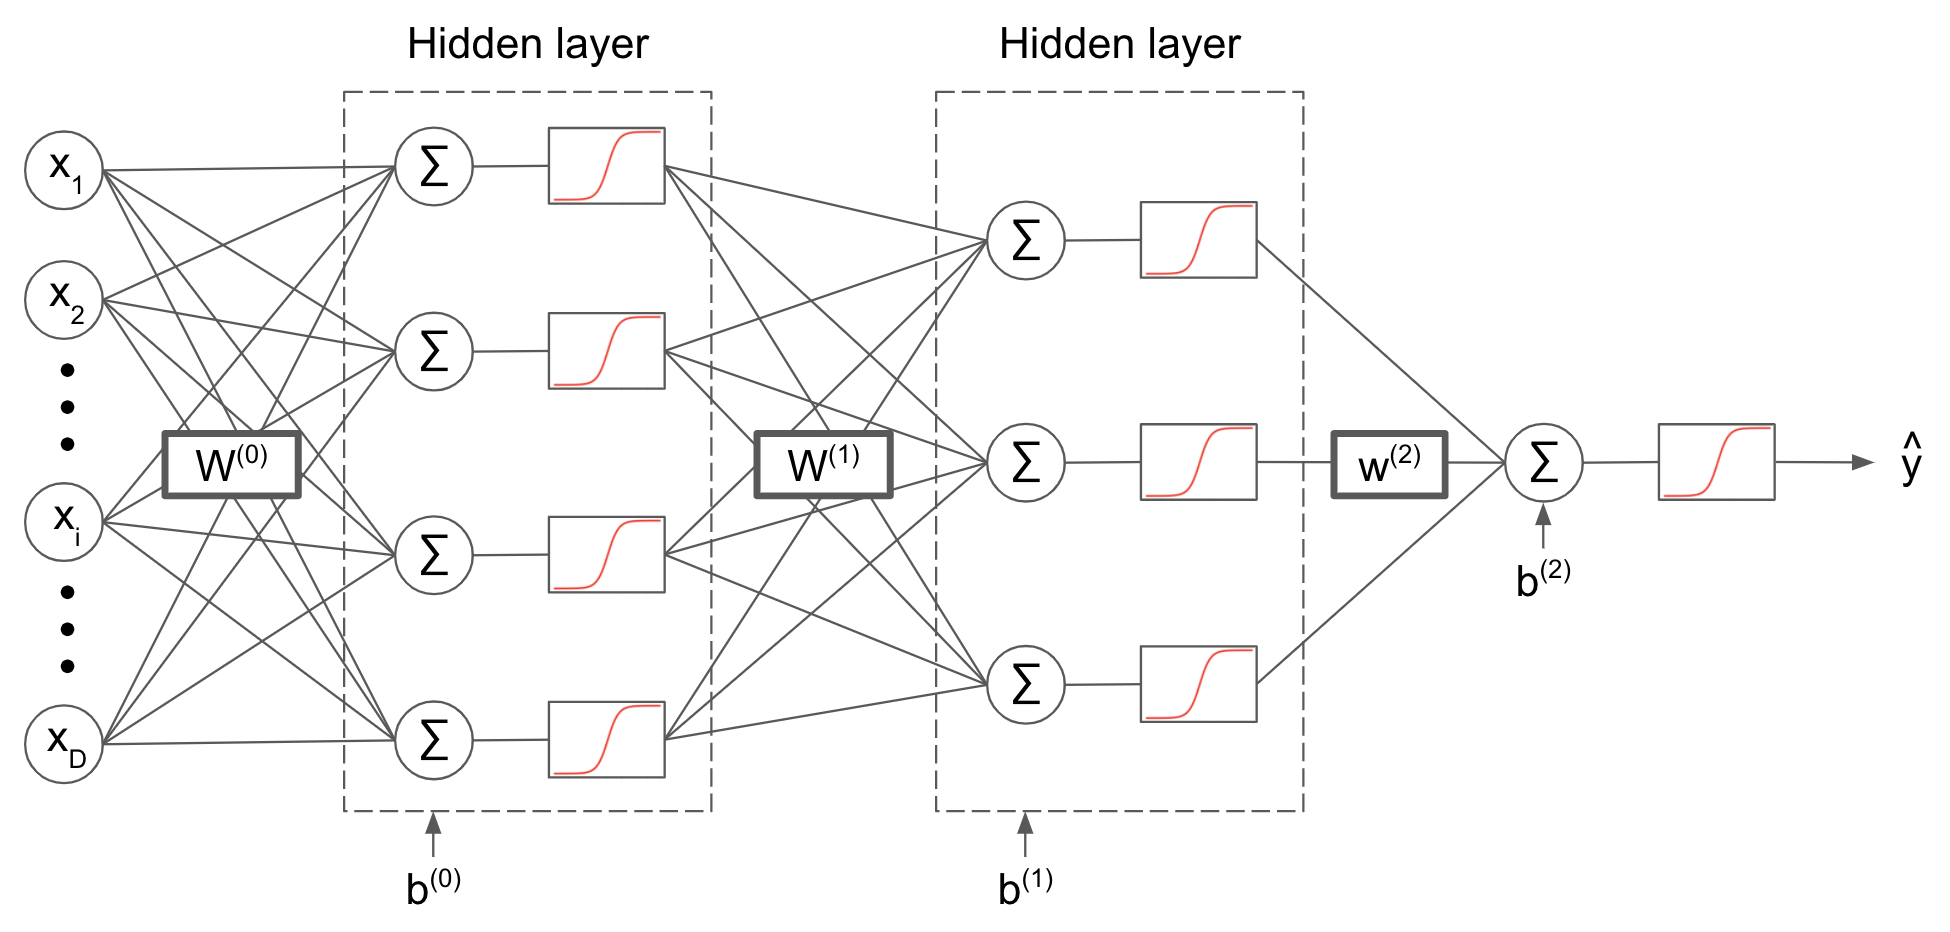
\includegraphics[width=0.8\textwidth]{../figures/ann_two_hidden_layers.png}
    \caption{Multilayer Perceptron with two hidden layer. Taken from \citep{RefWorks:webster2024week}}
    \label{fig:mlp}
\end{figure}

Figure~\ref{fig:mlp} demonstrates the potential that DNN's have for modelling higher order feature
interactions. By training the network by means of Stochastic Gradient Descent, it should be
possible to calculate the appropriate weight ($\mathbf{W}_l$) and bias ($\mathbf{b}_l$) parameters
in order capture the relevant high-order feature patterns in the data. As such, many CTR
modelling frameworks have been developed that use Deep Learning techniques to build upon and
imporved the previously discussed classical methods by incorporating Deep Neural Networks such
as the ML in the model architecture \citep{RefWorks:zhang2021deep}.

\subsection{Single vs Dual Tower Architectures}

\subsection{MLP Enhanced CTR models}

\subsubsection{Factorization-machine Supported Neural Networks}

\subsubsection{Wide and Deep}

The 
so-called \textbf{Wide and Deep} (W\&D) model was developed by \cite{RefWorks:cheng2016wide}:

\begin{equation}
    \label{eqn:wdl}
    f_{\Theta}^{W\&D} = \theta_0 + \sum_{k=1}^{\hat{n}} \theta_k \hat{\mathbf{x}}_k
    + f_{\Phi}^{MLP}(\tilde{\mathbf{x}})
\end{equation}

\begin{figure}[h]
\centering
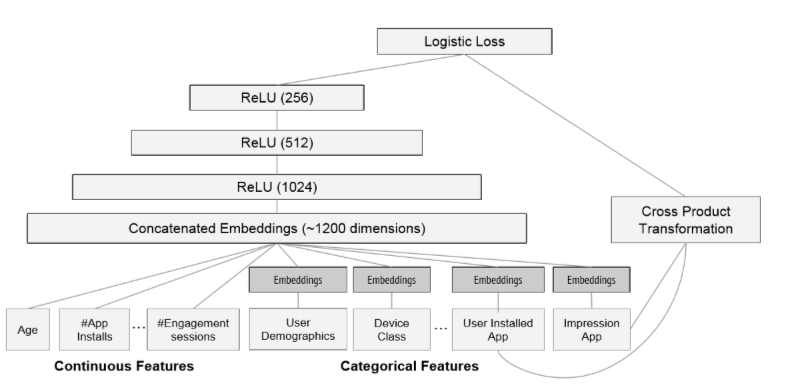
\includegraphics[width = 0.8\textwidth]{../figures/wdl.png}
\caption{Wide and Deep Model, as illustrated in \citep{RefWorks:shen2017deepctr:}}
\label{fig:wdl}
\end{figure}

Figure~\ref{fig:wdl} reveals that the W\&D model is composed with a Dual-Tower Architecture,
with a Deep Component and a Wide Component (shown on the left and right hand sides of Figure~\ref{fig:wdl}
respectively). The Deep Component is composed of a MLP with multiple hidden layers, each
with the Rectified Linear Unit (ReLU) activation function. The Wide Component is formulated
by the first two terms in equation~\ref{eqn:wdl}, and is composed of a simple linear transformation
of the input features. The key aspect of the Wide Component to take note of is that the 
linear transformation is not simply applied to the preprocessed features $\tilde{x}$,
but instead to these concatinated with a set of cross-product transformed features. In
other words:

\begin{equation}
\label{eqn:wdl-cross-product}
\hat{\mathbf{x}} = [\tilde{\mathbf{x}}, \upsilon_1({\tilde{\mathbf{x}}}),\ldots , \upsilon_P({\tilde{\mathbf{x}}})]
\end{equation}

Where $\upsilon_k({\tilde{\mathbf{x}}}) = \prod_{j=1}^{\tilde{n}}\tilde{x}_j^{c_{kj}}$
and $c_{kj} \in \{ 0, 1 \}$.

Consequentially of equation~\ref{eqn:wdl-cross-product}, the Wide Component \emph{memorizes}
the key feature interations that are defined by the specific \emph{cross-product transformations}
($\upsilon_{k}(\tilde{\mathbf{x}})$) \citep{RefWorks:cheng2016wide}. Meanwhile, the Deep Component captures any residual
signals that may not have been explicitly included in the manually defined cross-product transformations
\citep{RefWorks:zhang2021deep}.

\subsubsection{DeepFM}

\subsection{Feature Interaction Operator Models}

\subsubsection{Product Operators - Product Based Neural Network}

\subsubsection{Convolutional Operators - Feature Generation Convolutional Neural Network}

\subsubsection{Attention Operators - AutoInt}

\begin{figure}[h]
\centering
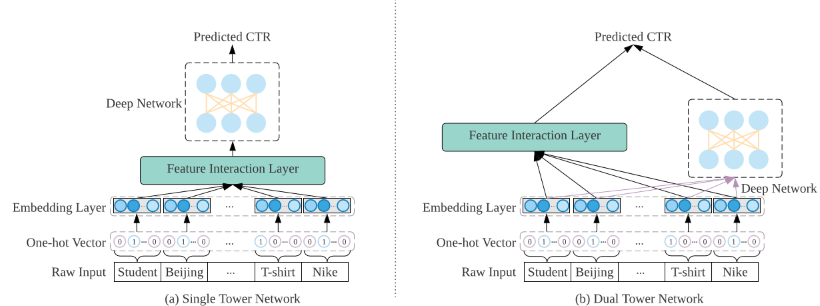
\includegraphics[width=\textwidth]{../figures/single_dual_dnn.png}
\caption{Deep Neural Network Architecture for CTR prediction. Image taken from \cite{RefWorks:zhang2021deep}}
\label{fig:dnn_architecture}
\end{figure}



\section{Deep Reinforcement Learning}

\subsection{Reinforcement Learning Basics: Markov Decision Processes and Dynamic Programming}

\subsection{Q-Learning and Deep Q-Learning}

\subsection{DRN: Deep Reinforcement Learning for News Recommendation}

In their survey, \citep{RefWorks:wang2024deep} describe how deep reinforcement learning combines 
the aforementioned feature extraction capabilities of DNN’s with the decision-making 
capability of reinforcement learning, which aims to learn an optimal state-action policy 
which maximizes the expected reward gained in a given environment. In the context of 
recommendation systems, a significant amount of research has been dedicated to formulating 
the recommendation problem as a Contextual Multi-Armed Bandit (MAB) problem setting, where 
the context consists of user, site and item features \citep{RefWorks:bouneffouf2012contextual-bandit,RefWorks:li2010contextual-bandit,RefWorks:zeng2016online}. 
However, a shortcoming for the MAB approach 
is that it does not explicitly model the future expected reward for the policy, which may 
be detrimental in the longer term \citep{RefWorks:zheng2018drn:}. Markov Decision Process (MDP) models 
solve for this issue by modelling the state-action progression as a Markov Process, allowing 
for the stochastic valuation of the future potential rewards for a given recommendation 
policy \citep{RefWorks:lu2016partially,RefWorks:mahmood2007learning}. DRN \citep{RefWorks:zheng2018drn:} is a MDP framework 
that leverages a Deep Neural Network to approximate the expected total user response for 
each recommendation at each state. The two major advantages of DRN are firstly that it is 
composed on the basis of a continuous state and action representation, meaning that it can 
be scaled to large and sparse datasets, and secondly that the proposed reward function 
consists of both the immediate reward (user click) as well as the future expected reward 
(long term user engagement), thereby allowing for better recommendations over a user’s 
lifetime.

\chapter{Deep CTR model Evaluation}
\label{chap:deep-ctr-model-evaluation}

\section{Model Selection Methodology}

As explained above, I will explore a number of deep learning models. I selected five popular models on the basis of the following criteria

\begin{itemize}
\item Competitive predition accuracy in the KDD12, Criteo and Avazu datasets as published on Papers with Code.
\item Ideally, I was looking for a representitive set of models for each model type as discussed in (Zhang et. al. 2021). Therefore I was looking for models that employed Product Interaction Opetators, Attention Operators and Factorization Machines as a basis.
\item The code for the model has to be accessible and intuitive to use.
\end{itemize}

On the basis of the above critea, I have chosen the following models to explore:

\begin{itemize}
\item Factorization Supported Neural Networks
\item Product Based Neural Networks
\item Wide and Deep
\item DeepFM
\item Automatic Feature Interaction (AutoInt)
\end{itemize}

In the section below, I briefly introduce each of the models, and evaluate against the benchmark datasets loaded and preprocessed above.

\section{Model Summaries}

\subsection{Shallow Models}

\subsubsection{Logistic Regression}


\subsubsection{Factorization Machines}

Factorization Machines were first introduced in \citep{RefWorks:rendle2010factorization} as
a model class that ``combines the advantages of Support Vector Machines (SVM) with factorization models''.
The model is able to capture the second order feature interactions in the data, which is a key advantage over
Logistic Regression. The model is defined as follows:

\begin{equation}
\label{eq:fm}
\hat{y}(\mathbf{x}) = w_0 + \sum_{i=1}^{n} w_i x_i + \sum_{i=1}^{n} \sum_{j=i+1}^{n} \langle \mathbf{v}_i, \mathbf{v}_j \rangle x_i x_j
\end{equation}

where $w_0$ is the bias term, $w_i$ are the weights for the $i$-th feature, $\mathbf{v}_i$ are the latent vectors for the $i$-th feature.
\cite{RefWorks:rendle2010factorization} shows that the learned biases and weights of the FM model can be
computed in linear time, ``and can be learned efficiently by gradient descent methods'', such as Stochastic Gradient Descent (SGD).


\subsection{Deep Models}

\subsubsection{Factirization Supported Neural Networks}

The first Deep Learning model that we will consider is the Factorization Supported
Neural Network (FNN) model proposed by \cite{RefWorks:zhang2016deep}. The model works by first training a Factorization Machine
model on the sparse-encoded categorical input features. It then uses the latent vectors learned by the FM model (see $\mathbf{v}_i$ in equation~\ref{eq:fm})
as inputs to a Neural Network, as shown in Figure~\ref{fig:fnn}. In doing so, the FNN model is effectively using the FM latent factors to initialize the embedding layer of the Neural Network.
The DNN is then able to learn the higher order feature interactions in the data, which the FM model is unable to capture.

\begin{figure}[h]
\centering
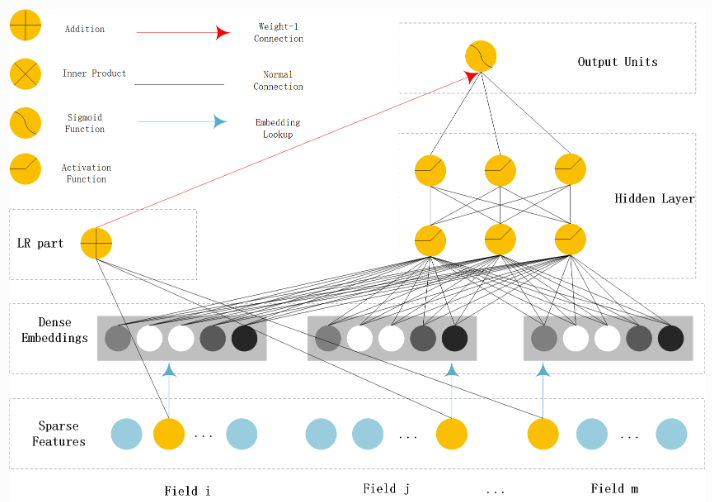
\includegraphics[]{../figures/fnn.png}
\caption{Factorization Supported Neural Network as proposed by \cite{RefWorks:zhang2016deep}. Image taken from \cite{RefWorks:shen2017deepctr:}}
\label{fig:fnn}
\end{figure}

\subsubsection{Product Based Neural Networks}

The Product Based Neural Network (PNN) model
proposed by \cite{RefWorks:qu2016product-based} is another Deep Learning
model that was developed around the same time as the FNN model. The key 
innovation of the PNN moel is the use of a pair-wisely connected Product Layer
after a field-wise connected embetting layer for the categorical features, as shown
in Figure~\ref{fig:pnn}. The Product Layer is able to directly model inter-field feature
interaction by means of either an inner product or outer production operation, and then further
distill higher feature inturactions by passing the output of the Product Layer through fully
connected MLP layers.


\begin{figure}[h]
\centering
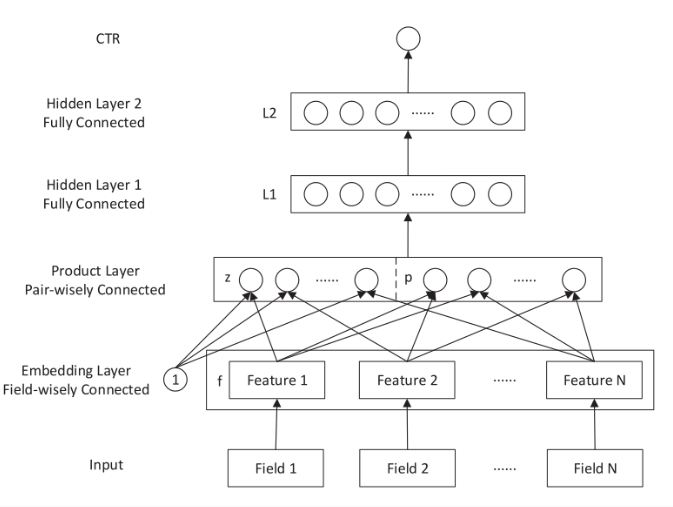
\includegraphics[]{../figures/pnn.png}
\caption{Product Based Neural Network as proposed by \cite{RefWorks:qu2016product-based}. Image taken from \cite{RefWorks:shen2017deepctr:}}
\label{fig:pnn}
\end{figure}


\subsubsection{Wide \& Deep Learning}

The Wide \& Deep Learning (WDL) model proposed by \cite{RefWorks:cheng2016wide} introduces the concept
of dual-tower model architecture \citep{RefWorks:zhang2021deep}. While both the FNN and the PNN models
generally tend to be constructed as a single fully connected DNN model, the Wide \& Deep model
consists of a wide component, consisting of a three layer Deep Neural Network that takes the concatinated
embedding vectors of the categorical features as input, and a deep component, consisting of a cross product
transformation of selected sparse categorical features. The logits from the wide and deep components are added
together to produce the final prediction. The architecture of the WDL model is shown in Figure~\ref{fig:wdl}.

\begin{figure}[h]
\centering
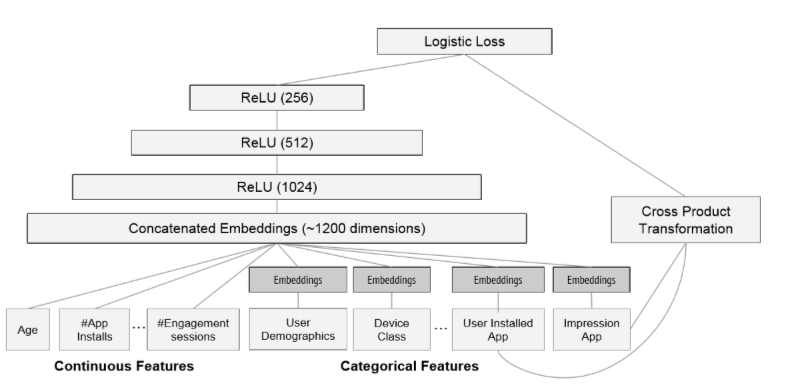
\includegraphics[]{../figures/wdl.png}
\caption{Wide \& Deep Learning model as proposed by \cite{RefWorks:cheng2016wide}}
\label{fig:wdl}
\end{figure}

The purpose behind the Dual-Tower architecture is to counteract the tendancy of the fully connected
single tower DNN models to lose the ability to capture low-order feature interactions \citep{RefWorks:zhang2021deep}.
The Wide component is able to capture the low-order feature interactions, while the Deep component is able to capture
the higher order feature interactions.

\subsubsection{DeepFM}

The DeepFM model proposed by \cite{RefWorks:guo2017deepfm:} can be thought of as an
imporvement of the aforementioned FNN \citep{RefWorks:zhang2016deep} and WDL \citep{RefWorks:cheng2016wide} models.
Like the FNN model, the DeepFM model usilises the Factorization Machine model \citep{RefWorks:rendle2010factorization}
to learn lower-order feature interactions. However, it also employs a dual-tower architecture
like the WDL model, with the Wide component being the FM model and the Deep component being a fully connected
DNN model. The DeepFM model is therefore able to avoid the limitations on capturing low-order
interactions that are inherent in the FNN model. In addition, due the the application of the FM to all
feature embeddings, the DeepFM model eliminates the need to choose which features 
to feed through the wide component, as is the case in the WDL model. The architecture of the DeepFM model is shown 
in Figure~\ref{fig:deepfm}.

\begin{figure}[h]
\centering
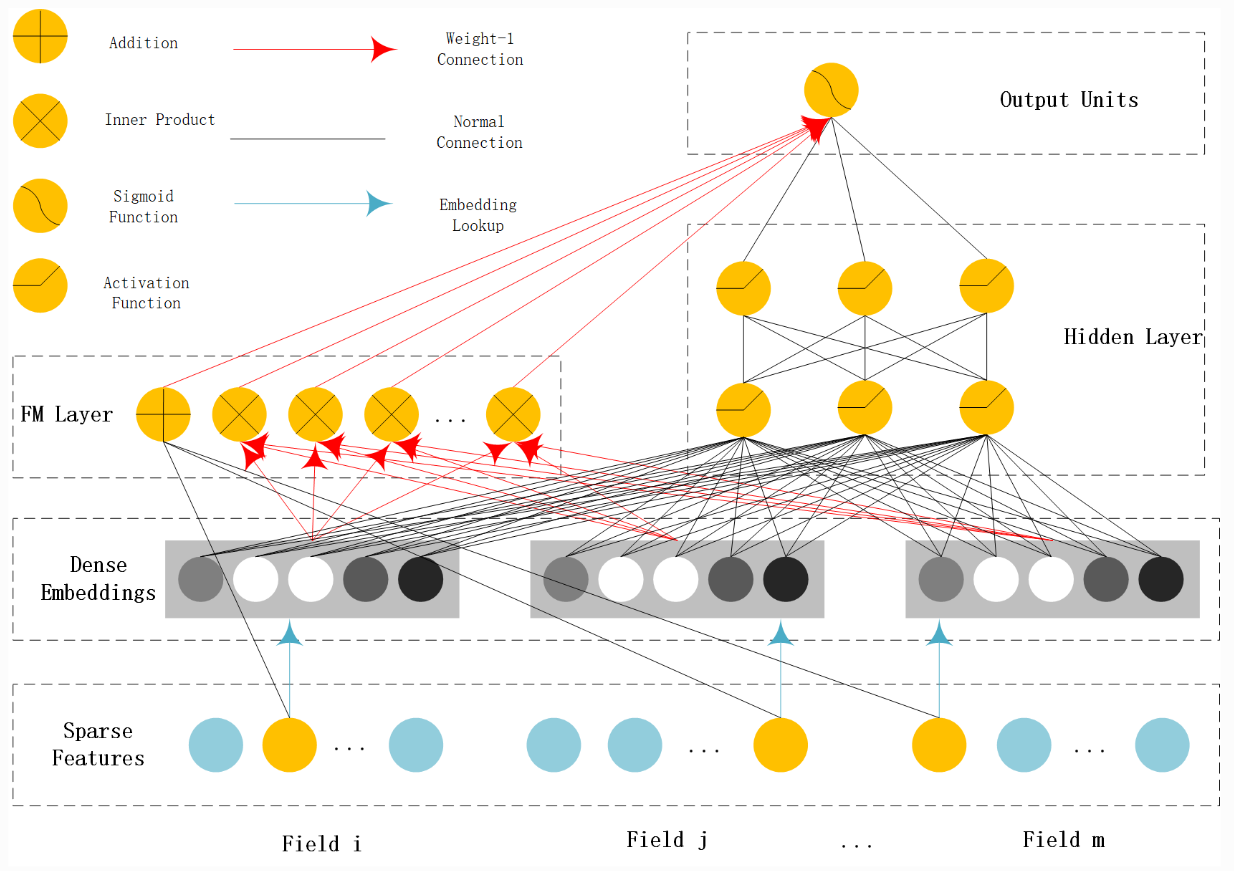
\includegraphics[width=\textwidth]{../figures/dfm.png}
\caption{DeepFM model as proposed by \cite{RefWorks:guo2017deepfm:}. Image taken from \cite{RefWorks:shen2017deepctr:}}
\label{fig:deepfm}
\end{figure}

%\subsubsection{Feature Generation by Convolutional Neural Network}

\subsubsection{Automatic Feature Interaction Learning}

The Autotomatic Feature Interaction Learning (AutoInt) model proposed by
\cite{RefWorks:song2019autoint} makes use of a multi-head self attention
network to model the important feature interactions in the data. The initial 
paper separates the model into three parts: an embedding layer, an interaction layer 
and an output layer. The embedding layer aims to project each sparse multi-value
categorical a and dense numerical feature into a lower dimensional space, as per the equation~\ref{eq:autoint-embedding}:

\begin{equation}
\label{eq:autoint-embedding}
\mathbf{e_i} = \frac{1}{q} \mathbf{V_i x_i}
\end{equation}

where $\mathbf{V_i}$ is the embedding matrix for the $i$-th field, $x_i$ is a multi-hot vector, and $q$ 
is the number of non-zero values in $x_i$. The interaction layer employs the multi-head
mechanism to determine which higher order feature interaction are meaningful in the data. This not only
improves the efficiency of model traning, but it also improves the model's explainability. Lastly,
the output layer is a fully connected layer that takes in the concatinated output 
of the interaction layer, and applies the sigmoid activation function to produce the final prediction.
The architecture of the AutoInt model is shown in Figure~\ref{fig:autoint}.

\begin{figure}[h]
\centering
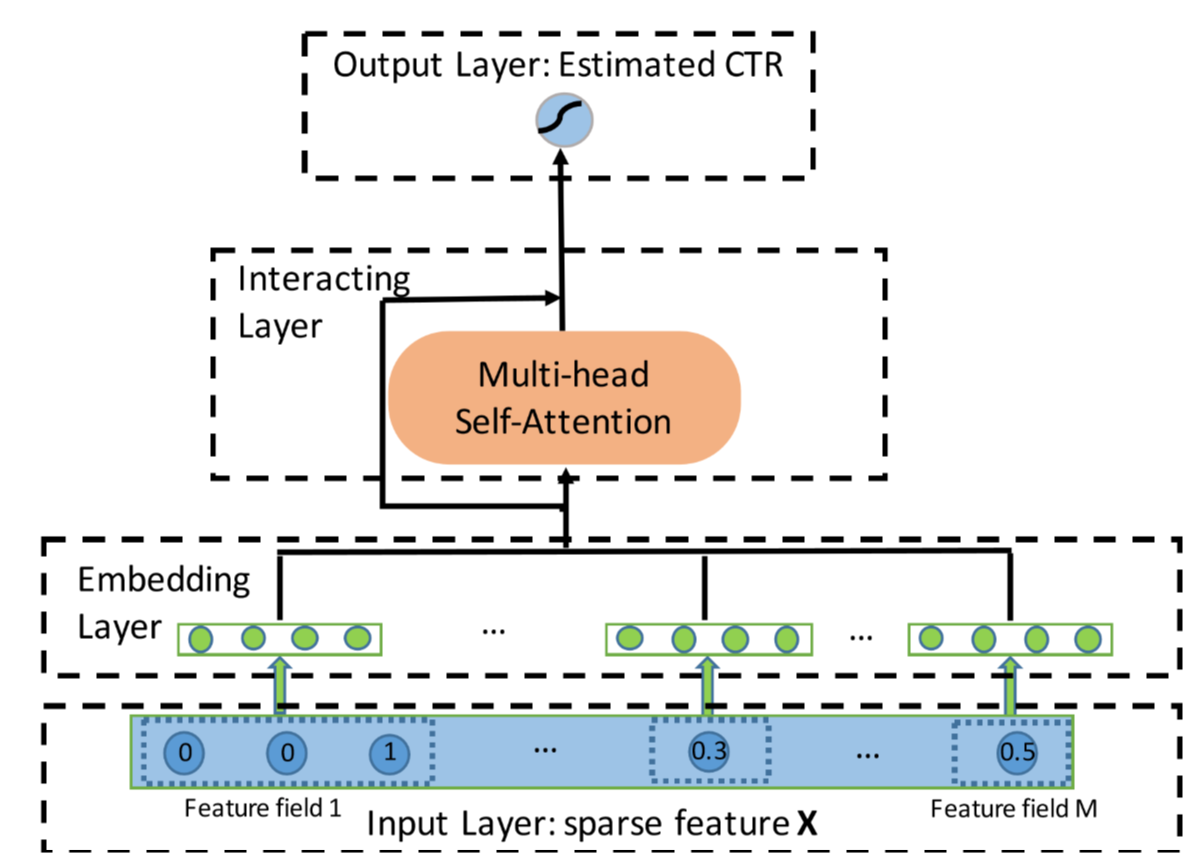
\includegraphics[width=\textwidth]{../figures/autoint.png}
\caption{AutoInt model as proposed by \cite{RefWorks:song2019autoint}}
\label{fig:autoint}
\end{figure}

\section{Experiment Setup}

\subsection{Datasets and Preprocessing}

\subsection{Evaluation Metrics}

\subsection{Hyperparameter Selection}

\section{Deep CTR Model Results}

\chapter{Deep Reinforcement Learning for Ad Personalization}
\label{chap:deep-rl-for-ad-personalization}

\section{DeepCTR-RL Framework}

\subsection{Model Framework}

\subsection{Feature types}

\subsection{Double Deep Q-Learning Network}

\subsection{Exploration}

\subsection{Experience Replay}

\section{Experiment Setup}

\subsection{Dataset and Preprocessing}

\subsection{Evaluation Metrics}

\subsection{Hyperparameter Selection}

\section{Deep CTR-RL Results}

\chapter{Discussion}
\label{chap:discussion}

Discussion goes here.

\chapter{Conclusion}


Conclusion goes here. 





\clearpage
 %% reset page counter and start appendix pages with A
\pagenumbering{arabic}
\renewcommand*{\thepage}{A\arabic{page}}

%% Appendix goes here
\appendix
%
\chapter{Appendix}

\section{Abbreviations and Acronyms}
\label{app:acronyms}

\begin{table}[ht]
    %\centering
    \begin{tabular}{|l|l|l|}
      \hline
        \textbf{Term} & \textbf{Definition} & \textbf{Reference} \\
      \hline
        LR& Logistic Regression & \\
        FM & Factorization Machine & \\
        FFM & Field-Aware Factorization Machine & \\
        DNN & Deep Neural Network & \\
        MLP & Multilayer Perceptron & \ref{ref:mlp} \\
    \hline
    \end{tabular}
\end{table}


\section{Notation}
\label{app:notation}

\begin{table}[ht]
    %\centering
    \begin{tabular}{|l|l|l|}
      \hline
        \textbf{Symbol} & \textbf{Definition} & \textbf{Reference} \\
      \hline
        $\mathbf{x}$& Feature vector, before pre-processing &\\
        $n$ & the number of features in $\mathbf{x}$ &\\
        $x_i$& The $i$-th feature in $\mathbf{x}$ &\\
        $\mathbf{x_i}^{OH}$ & One-hot encoded vector representation of categorical feature $i$ &\\
        $\mathbf{e}_i$ & Embedded vector representation of categorical feature $i$ & \\
        $z_i$ & Mean and variance standardized value for feature $i$ from $\mathbf{x}$ &\\
        $\tilde{\mathbf{x}}$ & $\mathbf{x}$ after catigorical embedding and numerical standardization. &\\
        $f$ & Pre-sigmoid classification function &\\
        $\Theta$ & Parameter vector for $f$ & \\
    \hline
    \end{tabular}
\end{table}


%%References part of appendices
% References: modify the file refs.bib
\bibliographystyle{plainnat}
\bibliography{refs}


\end{document}
